\documentclass[12pt]{third-rep}
%% The third-rep class and this starter kit were written by 
%% Graham Gough <graham@cs.man.ac.uk>
%% If you have any comments or questions regarding this document,
%% please post them to the local newsgroup man.cs.tex.
%%
%% More information about LaTeX in general and the local setup in
%% particular can be found on the web at 
%% http://csis.cs.manchester.ac.uk/software/contrib/latex
%%
%%%%%%%%%%%%%%%%%%%%%%%%%%%%%%%%%%%%%%%%%%%%%%%%%%%%%%%%%%%%%%%%%%%%%%%%

\usepackage{url} % typeset URL's sensibly
\usepackage{hyperref}
\hypersetup{
    colorlinks=true,
    linkcolor=blue,
    filecolor=magenta,      
    urlcolor=cyan,
}

% \usepackage{pslatex} % Use Postscript fonts

\usepackage[ruled]{algorithm2e}

% maths definitions
\usepackage{amsthm}
\theoremstyle{plain}
\newtheorem{thm}{Theorem}[chapter]
\theoremstyle{definition}
\newtheorem{defn}[thm]{Definition}

% maths symbols
\usepackage{amsmath}
\usepackage[adobe-utopia]{mathdesign}
\let\mathcal\undefined
\DeclareMathAlphabet{\mathcal}{OMS}{cmsy}{m}{n}

%% This defines the title
\title{Reinforcement learning for a learnable agent\\
in classic arcade games}
%% and author
\author{Sean J Parker}
%% and supervisor
\supervisor{Dr. Konstantin Korovin}
%% and the year of the report
\reportyear{2020}

%% this defines the file that contains the text of the abstract, there
%% must be one of these by the time you submit your report.
\abstractfile{abstract.tex}

%% this defines the file that contains the acknowledgements (it can be
%% omitted if you don't feel like thanking anyone
\thanksfile{merci.tex}

%% Uncomment the following lines if you want to include the date as a
%% header in draft versions. See the documentation for fancyhdr for
%% more ways of modifying headers (texdoc fancyhdr will show you the
%% docs) 

%\usepackage{fancyhdr}
%\pagestyle{fancy}
%\lhead{}  % left head
%\chead{Draft: \today} % centre head
%\lfoot{}
%\cfoot{\thepage}
%\rfoot{}

%% The following line sets up the use of PostScript fonts rather
%% than the standard bitmapped fonts.
\usepackage{pslatex}

%% Uncomment the following line if you want to change the name of the
%% Bibliography to References
\renewcommand{\bibname}{References}

\usepackage{listings}

%% End of preamble, the actual document starts here
%%

\begin{document}

%% This actually creates the title and abstract pages
\dotitleandabstract

%% Generate contents etc
\tableofcontents
\listoffigures
\listoftables

%% These include the actual text
\chapter{Introduction}
\label{cha:intro}
My project aims to implemented and compare some of the reinforcement learning algorithms that have been used to play classic Atari 2600 games. It also compares the results of different tests with these algorithms such as varying the hyperparameters of the network. By observing the effects on the trained agents\footnote{Agent. In this case, agent refers to a trained neural network that takes actions in a chosen environment.} when the hyperparameters are changed we can deduce a set of optimal values such that the networks can play three different Atari 2600 games. Overall, the main features of the project are the following:
\begin{itemize}
  \item Agents with raw pixel data as input, outputting a set of values for the best action.
  \item Agents attempt to find an optimal model of the environment without any prior knowledge.
  \item Visualization of the agents ``brain'' to provide insight into what information the agent is learning.
\end{itemize}

Concerning the first point above, there are two ways in which you can provide inputs to agents that play games. The first (and often simplest) option is by using values from specific locations in RAM\footnote{In this case, RAM refers specifically to the in-game memory.}. If we take the game Pong as an example, we could take information such as the enemy paddle y-position, the ball x,y-position, the players paddle y-position and finally the score. By having this information without any processing required, it helps to reduce the state space.

On the other hand, another option is to take as input the raw pixels from the game, it makes it more difficult to play the game as we need to interpret the pixels to deduce all the information to make optimal moves. This is the approach we take as it more closely simulates how a human player would observe information from the game. Additionally, this project also aims to implement a variety of methods that are described in \ref{dsgn:sec:qlearning} and \ref{dsgn:sec:qlearning:qextra}; the simplest of which is a method called Q-Learning and then further improvements to the Q-Learning called Double Q-Learning and Duelling Q-Learning.

Finally, this project describes methods by which it is possible to visualise the agents ``brain'', there has been much research in recent years into methods to visualise high-dimensional data when investigating neural network and this project explores and implements one such method that will visualise what information the agent has learnt about the environment.

\section{Motivation}
\label{intro:sec:moti}
Over the past 10 years, there has been significant improvement in the RL (reinforcement learning) algorithms. One reason is that computing power has become cheaply available by using discrete graphics cards. For example, for my project, I used an Nvidia GeForce GTX 1070 that provides 1920 CUDA cores that can be used to accelerate training of neural networks. Despite this, RL algorithms are massively computationally expensive and hence take a long time to train.

Over recent years one of the pioneers in this area is DeepMind, which was acquired by Google in 2014, and they developed the DQN (deep q-network) algorithm in 2013 which they demonstrated could learn directly from the raw pixel data of games to achieve either human-level or super-human level performance.

This research was expanded upon by DeepMind and OpenAI which is based on the original DQN by DeepMind. This research focused on trying to approximate a Q-function and thereby infer the optimal policy. On the other hand, there has recently been a focus on other methods such as A3C and PPO which instead seek to directly optimise in the policy space of the environment.

\section{Objectives}
\label{intro:sec:obj}
Further to what was described in section \ref{cha:intro}, there were a few main objectives of the project. Firstly, I chose three games on which I decided to train the agents, Pong, Breakout, and Space Invaders which are shown below in Figure \ref{fig:atari-screenshot}.

\begin{figure}[htbp]
  \centering
  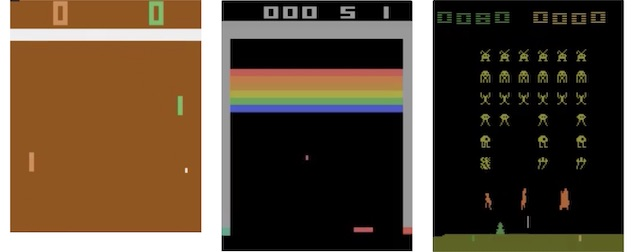
\includegraphics[width=0.7\textwidth]{chapters/chapter1/images/atari-combined.jpg}
  \caption{Screenshots of Pong, Breakout, Space Invaders (left to right).
    \label{fig:atari-screenshot}
  }
\end{figure}

Secondly, having a method to explore the internals of a trained agent can provide further insight into what the agent is trying to learn. A major benefit for this approach is that a researcher could use this information to determine, for example, where the agent has learnt to focus on the frame based on the filter activation maps. Additionally, it also can point towards poor hyperparameter choice such as a high learning rate when the layers have many dead filters. More discussion of these techniques is provided in Section \ref{bg:sec:cnn-vis}.

\section{Report structure}
\label{intro:sec:report_struc}

This report is divided into three main sections. First, describing the background of the problem and the history of the methods/techniques that underpin reinforcement learning and neural networks. Further, a section providing a detailed discussion of the project design and motivating the choice of some of the decisions made in this project. After that, a section discussing the implementation of the project and system design. Penultimately, we will discuss the evaluation of the project with a comparison of the different techniques and critical analysis. Finally, this report ends with a personal reflection on this project.

\section{Impact of COVID-19}
COVID-19 has caused widespread disruption across the faculty and University as a whole, and unfortunately, it also impacted my plans for the Semester. The circumstances surrounding the pandemic lead to uncertainty around whether it was safe to be at University and made it more difficult to maintain the required level of focus and motivation on the project, mainly as I was concerned about if I should travel home or have the possibility of being quarantined in University accommodation. On the other hand, I know that many people were more affected than I, in comparison my situation was much less disrupted than others.
\chapter{Background}
\label{cha:bg}

\section{Reinforcement learning}
\label{bg:sec:rl}

\section{DQN on Atari 2600}
\label{bg:sec:dqn}

\section{CNN Visualisation}
\label{bg:sec:cnn-vis}
\chapter{Design}
This section will cover the details of the methods and algoithms that were used in the implementation of the project. The previous section covered the history of some of these techniques which were imperative for building the foundation of the methods described in this chapter.

Deep Q-Networks and its enhancements have the majority of focus, as it is the basis of the project. Below is a table of the different experiments and the methods that were used in order to produce the best solution for each tested environment.

\begin{table}[ht!]
	\begin{center}
		\begin{tabular}{|c|c|c|}
			\hline
			Network   & Algorithm                  & Environment    \\
			\hline
			CNN + MLP & Q-Learning                 & Pong           \\
			CNN + MLP & Q-Learning                 & Breakout       \\
			CNN + MLP & Duelling Double Q-Learning & Space Invaders \\
			\hline
		\end{tabular}
		\caption{Best performing method in given environment}\label{table:design:algo-experiment}
	\end{center}
\end{table}

\section{Markov decision process}
\label{dsgn:sec:mdp}
This section will describe some of the basics of Markov decision processes (MDP), they are the foundation of the reinforcement learning methods that will be described later in this chapter. First, we need some mathematical definitions of MDPs, these are from David Silver's excellent lecture series on Reinforcement Learning.

Markov decision processes are just markov reward processes with decisions, i.e. At each state $S_t$, we have a finite set of actions to choose from in order to get to a new state $S_{t+1}$.

\begin{defn}
	A Markov decision process is a tuple $\langle \mathcal{S}, \mathcal{A}, \mathcal{P}, \mathcal{R}, \gamma \rangle$.
	\begin{itemize}
		\item $\mathcal{S}$, finite set of states
		\item $\mathcal{A}$, finite set of actions
		\item $\mathcal{P}$, state transition probability matrix,~\\$\mathcal{P}_{ss'}^a = \mathbb{P}[S_{t+1}=s'|S_t=s, A_t=a]$
		\item $\mathcal{R}$, reward function, $\mathcal{R}_s^a = \mathbb{E}[R_{t+1}|S_t=s,A_t=a]$
		\item $\gamma$ discount factor, $\gamma\in[0,1]$
	\end{itemize}
\end{defn}

The definition above defines a Markov decision process, which we use as a basis for describing the methods in reinforcement learning. In order to illustrate the idea, let us consider the game of Pong. For simplicity, assume we can encode each frame of the game into the set of states $\mathcal{S}$. In order to play the game, we need to know what the best action to take would be at each frame of the game to move the paddle under the ball, hitting the ball back and (hopefully) scoring a point.

Given a frame of the game $S_t$ and the set of actions we can choose from $A_t$, we are going to try and maximise our future (expected) reward using the reward function $\mathcal{R}_{S_t}^{A_t}$. We want to choose the best action $a$, that will result in the maximum future reward. It is important that we don't look at immediate rewards only, since, in Pong we don't get the point until we have hit the ball back to the other side.

In order to look at future rewards, we use the discount factor $\gamma$. When $\gamma$ is close to zero, we are ``\textit{myopic}'' in our evaluation (we only look for short-term rewards). However, as $\gamma$ gets closer towards 1, we are ``\textit{far-sighted}'' in our evaluation.

Overall, we need to know a strategy that provides the best action to take in a given state which maximises the expected total reward. This is called a \textit{policy}, denoted by $\pi$.

\begin{defn}
	A \textit{policy} $\pi$ is a distribution over actions given states,
	\begin{center}
		$\pi(a~|~s)=\mathbb{P}[A_t=a~|~S_t=s]$
	\end{center}
\end{defn}

The policy of an agent fully describes the behaviour of the agent (TODO: add ref) which only depends on the current state, not the history. In order to describe the optimal policy for an agent to follow, we first need some more definitions.

\begin{defn}
	$G_t$ is the total discounted reward for time-step $t$
	\vspace*{-7mm}
	\begin{center}
		$$G_t = R_{t+1} + \gamma R_{t+2} + \dots = \sum_{k=0}^{\infty}\gamma^{~k}~R_{t+k+1}$$
	\end{center}
\end{defn}

\begin{defn}
	\label{action-value-func}
	The \textit{action-value} function $q_\pi(s,~a)$ is expected return starting from state $s$, taking action $a$, following policy $\pi$
	\begin{center}
		$q_\pi(s,~a)=\mathbb{E}_\pi[G_t~|~S_t=s,~A_t=a]$
	\end{center}
\end{defn}

\noindent In addition to the action-value function $q_\pi(s,~a)$ we also define the state-value function for a given state $s$.

\begin{defn}
	\label{state-value-func}
	The \textit{state-value} function $v_\pi(s,~a)$ is the expected value of a being in a given state $s$ while under a policy $\pi$

	\begin{center}
		$v_\pi(s,~a) = \mathbb{E}_{a\sim \pi(s)}\left[q_\pi(s,~a)\right]$
	\end{center}
\end{defn}

\begin{defn}
	The \textit{optimal action-value} function is denoted by $q_*(s, a)$ and is the maximum action-value function over all possible policies
	\vspace*{-7mm}
	\begin{center}
		$$q_*(s,~a)=\max_\pi q_\pi(s,~a)$$
	\end{center}
\end{defn}

Once we have found the optimal action-value function we consider the MDP ``solved''. Additionaly, we know that we can, given some state, take actions that will lead to the highest possible future reward.

\subsection{Markov property}
With Markov decision processes we assume that in each state, we have all the information we require in order to produce an optimal action. However, in games such as Pong and Breakout, we may not necessarily have all the information we require at a single time. For example, Figure \ref{fig:breakout-brick-fig} shows a screenshot of the Atari game Breakout. In this situation, we cannot decern the optimal action given only this frame as the ball has only just hit the brick.

\begin{figure}[htbp]
	\centering
	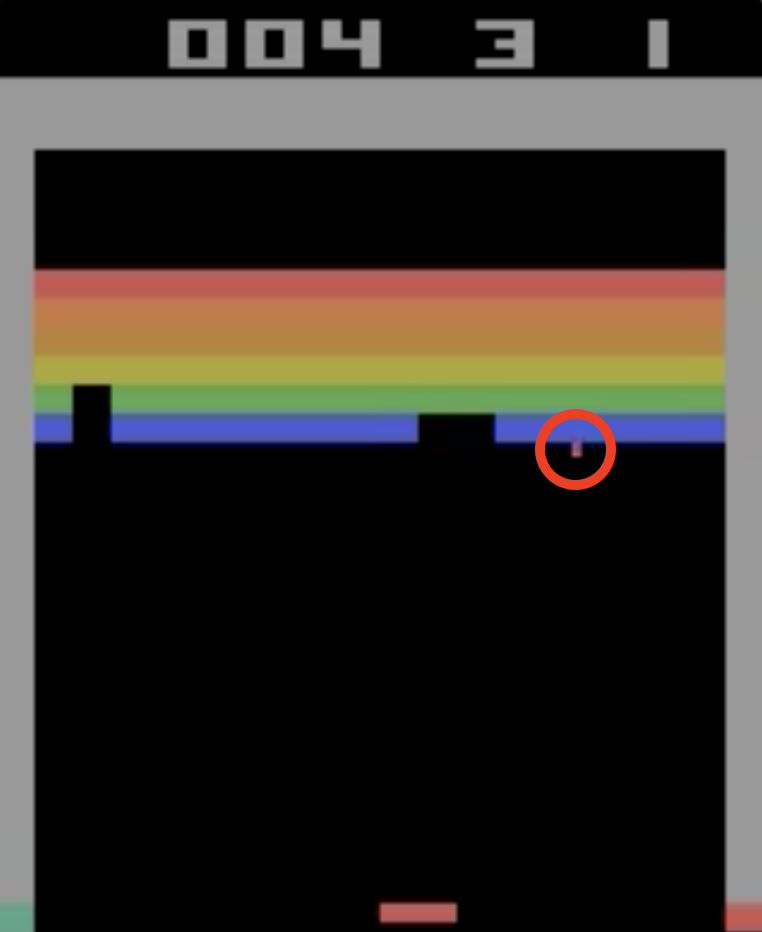
\includegraphics[width=0.30\textwidth]{chapters/chapter3/images/breakout.png}
	\caption[Screenshot of single breakout frame]{Screenshot of a breakout frame with the ball highlighted showing it just before the brick is destrotyed. The ball is highlighted using a red circle.
		\label{fig:breakout-brick-fig}
	}
\end{figure}

In order to solve this problem, in we store a small rolling history of $k$ states (where typically, $k = 4$) called the ``\textit{frame-stack}''. During forward passes through the network we pass the whole frame-stack to the network. This provides a history of frames to the network which has been shown, experimentally, to improve the learning of the algorithm.

\section{Reinforcement learning}
\label{dsgn:sec:rl}
Following on from the previous section on Markov decision processes, this section decribes Reinforcement learning and how these two methods are tightly connected to each other.

In its basic form, RL can be modelled graphically as shown in Figure \ref{fig:rl-diagram}. The agent gets the state from the environment, using its policy, it chooses an action to take -- updating the environment. The environment then produces some new state and a reward signal which the agents uses the pick the next action.

\begin{figure}[htbp]
	\centering
	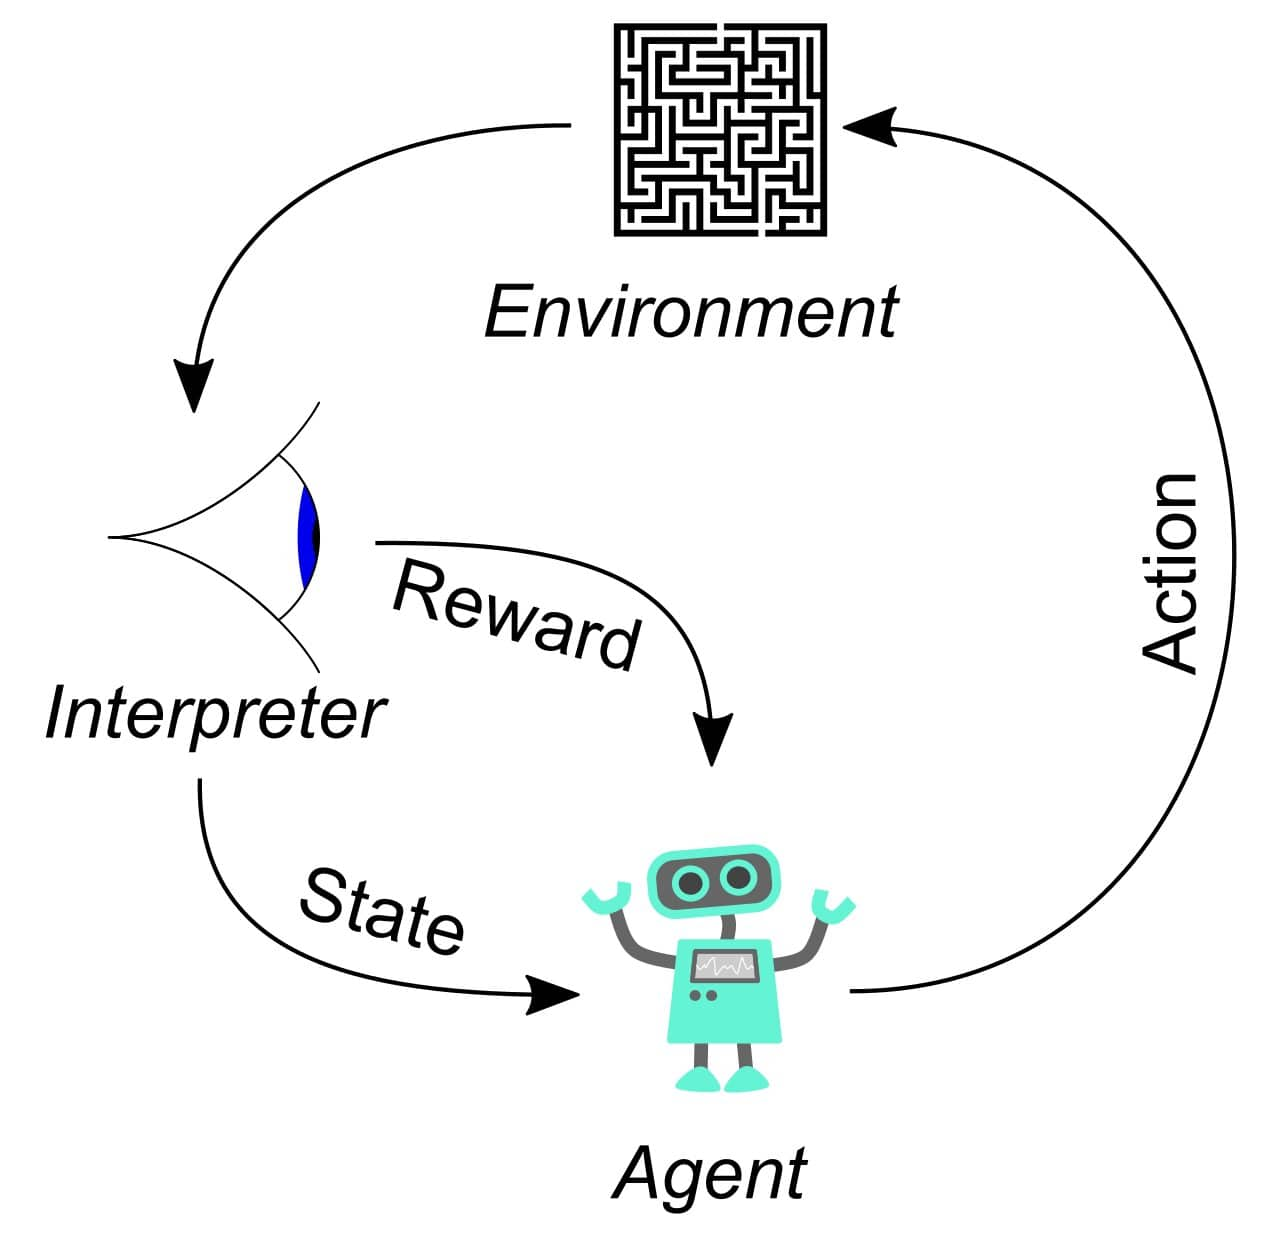
\includegraphics[width=0.35\textwidth]{chapters/chapter3/images/rl.jpg}
	\caption{Diagram of reinforcement learning
		\label{fig:rl-diagram}
	}
\end{figure}

\subsection{Exploration vs Exploitation}
\label{dsgn:sec:rl:expt-v-explor}
A key idea in RL is the problem of exploration vs exploration. This means that if we have an ennvironment, and a policy that dictates how we should navigate the environment, should always follow the policy, or should we deviate and try to find a better path resulting in a higher reward.

In this project we follow a method called $\epsilon$-greedy in which we explore forever, but with a linearly decreasing probability (denoted by $\epsilon$) of random actions, this is decreased over a predefined number of timesteps. Below is the method for choosing the actions.

\begin{center}
	\begin{itemize}
		\item Choose random action with probability $\epsilon$
		\item With probability $1 - \epsilon$ select \vspace*{-9.25mm} action = $$\argmax_{a \in \mathcal{A}}~\hat{Q}(a)$$
	\end{itemize}
\end{center}

Although $\epsilon$-greedy is one of the simplest and a naïve method, it is suprisingly effective in exploring the environment and produces high scoring models. In fact, this method was used in the original DQN paper by V.Mnih et al. in which they scored better than human averages in the majority of Atari 2600 games.

In the area of reinforcement learning, there are some more advanced methods such as Upper Confidence Bounds (UCB) and Thompson Sampling. However, these Bayesian-based methods are not implemented/explored in this project and is left for future work.

\newpage

\section{Q-Learning}
\label{dsgn:sec:qlearning}
Q-Learning is a model-free algorithm that is used to solve, iteratively, the Bellman equation for the MDP. By model-free we mean that the algorithm does not require a model of the environment, therefore it can easily handle stoachastic rewards. The method was introduced in 1989 by Chris Watkins in his PhD thesis titled ``\textit{Learning from delayed rewards}''.

We can use Q-Learning in order to approximate $q_*(s, a)$, this produces the optimal policy $\pi$ based on the Q-values. The Q-Learning algorithm stores the state-action values in a large table of values, as represented below in Table \ref{table:design:qtable}. For each possible state that the enviroment can produce, we store a single value (Q-value) for each action that can be performed in that state. These Q-values represents the `\textit{quality}`'' of being in a state $s$ and taking action $a$.

\begin{table}[htb!]
	\centering
	\begin{tabular}{|
			>{\columncolor[HTML]{468291}}c |
			>{\columncolor[HTML]{7EB1BD}}c |
			>{\columncolor[HTML]{EFEFEF}}l |
			>{\columncolor[HTML]{EFEFEF}}l |
			>{\columncolor[HTML]{EFEFEF}}l |
			>{\columncolor[HTML]{EFEFEF}}l |}
		\hline
		\multicolumn{2}{|l|}{\cellcolor[HTML]{EFEFEF}}                           &
		\multicolumn{4}{c|}{\cellcolor[HTML]{4682E6}{\color[HTML]{FFFFFF} Actions}} \\ \cline{3-6}
		\multicolumn{2}{|l|}{\multirow{-2}{*}{\cellcolor[HTML]{EFEFEF}Q-Table}}  &
		\multicolumn{1}{c|}{\cellcolor[HTML]{7AA1E1}{\color[HTML]{FFFFFF} NOOP}} &
		\multicolumn{1}{c|}{\cellcolor[HTML]{7AA1E1}{\color[HTML]{FFFFFF} FIRE}} &
		\multicolumn{1}{c|}{\cellcolor[HTML]{7AA1E1}{\color[HTML]{FFFFFF} LEFT}} &
		\multicolumn{1}{c|}{\cellcolor[HTML]{7AA1E1}{\color[HTML]{FFFFFF} RIGHT}}   \\ \hline
		\cellcolor[HTML]{468291}{\color[HTML]{FFFFFF} }                          &
		{\color[HTML]{FFFFFF} 0}                                                 &
		0                                                                        &
		0                                                                        &
		0                                                                        &
		0                                                                           \\ \cline{2-6}
		\cellcolor[HTML]{468291}{\color[HTML]{FFFFFF} }                          &
		{\color[HTML]{FFFFFF} 1}                                                 &
		-2.3452                                                                  &
		-1.8375                                                                  &
		-2.3634                                                                  &
		-1.5463                                                                     \\ \cline{2-6}
		\cellcolor[HTML]{468291}{\color[HTML]{FFFFFF} }                          &
		{\color[HTML]{FFFFFF} \vdots}                                            &
		\vdots                                                                   &
		\vdots                                                                   &
		\vdots                                                                   &
		\vdots                                                                      \\ \cline{2-6}
		\multirow{-4}{*}{\cellcolor[HTML]{468291}{\color[HTML]{FFFFFF} States}}  &
		{\color[HTML]{FFFFFF} 128}                                               &
		2.4456                                                                   &
		1.2345                                                                   &
		6.3462                                                                   &
		3.8356                                                                      \\ \hline
	\end{tabular}
	\caption[Q-Table Example]{Example of how state-action pairs are stored in a Q-Table (NOOP abbreviates `No action/No operation')}\label{table:design:qtable}
\end{table}

Since the Q-Learning algorithm is iterative, at each timestep, we need to update the Q-value corresponding to the occupied state and the action we took. In Chapter \ref{dsgn:sec:dql} this idea will be expanded upon, by using neural networks as a function approximator, replacing the need to store the whole table of Q-values. Algorithm \ref{algo:qlearning} shows how the algorithm is implemented in order to both, predict the next action to take, and updating the Q-table. In order to update the Q-values for each state we use the Q-value update equation which is shown below.

\begin{defn}
	$$Q_{t+1}(s_t, a_t) = Q_t(s_t, a_t) + \alpha(R_t + \gamma \max_a Q(s_{t+1}, a) - Q(s_t, a_t))$$
	\begin{itemize}
		\item $Q(s, a)$, q-value for state-action pair
		\item $\alpha$, learning rate
		\item $R$, immediate reward from enviroment
		\item $\gamma$ discount factor, $\gamma\in[0,1]$
		\item $max_a Q(s_{t + 1},~a)$, estimate of optimal future reward
	\end{itemize}
\end{defn}

A major issue with Q-Learning is that since we perform a maximisation of all future rewards when updating the Q-values, this can lead to the algorithm over-estimating the quality of actions and slowing down the learning. During training, we use the same Q-function in order to both produce the expected maximum action-value of future rewards and, select the best possible action in the current state.

\begin{algorithm}[H]
	\SetAlgoNoLine
	\DontPrintSemicolon
	Initialize action-value function $Q$ with random values\;
	\For{timestep = 1}{
	Initialise S\;
	\While{S is not done state}{
	With probability $\varepsilon$ choose random action $a_t$\;
	Else, pick $a_t = \max_{a}Q(s_t, a)$\;
	Take action $a_t$ and observse reward $r_t$ and state $s_{t + 1}$\;
	$Q(s, a) = Q(s_t, a_t) + \alpha(R + \gamma~max_{a}Q(s_{t + 1}, a) - Q(s_t, a_t))$\;
	Update $s_t = s_{t + 1}$
	}
	}
	\caption{Tabular Q-Learning}
\end{algorithm}

As shown above, we can use Q-learning to find the optimal policy by storing all the $q_*(s, a)$ values. However, in practise we run into a issue with the size of the Q-table in that it quickly becomes too big to store in memory. This issue is especially prevalent for large MDPs such as those from Atari games due to the raw pixel input. In order to handle the high-dimensonal input from the games, we can instead use a function approximator to estimate the values of $q_*(s, a)$. This idea will be developed in Section \ref{dsgn:sec:dql} where RL is combined with Deep Learning.

\section{Deep Learning}
\label{dsgn:sec:dl}
This section will describe the basics used in the project for Deep Learning and some of the techniques used in order to construct the Deep Q-Networks discussed in Section \ref{dsgn:sec:dql}.

\subsection{Multi-layer perceptron (MLP)}
\label{dsgn:sec:dl:mlp}
The main technique that underpins most of the artificial neural networks (ANN) that are used today is how we combine single neurons to for networks of neurons. Figure \ref{fig:neuron} shows how we model an artificial neuron with weights and activation functions, this is supposed to loosely model how neurons work inside the brain. The input connections are acting in place of synapses which connect together to form networks.

\begin{figure}[ht!]
	\centering
	\begin{tikzpicture}[
		init/.style={
				draw,
				circle,
				inner sep=2pt,
				font=\Huge,
				join = by -latex
			},
		squa/.style={
				draw,
				inner sep=2pt,
				font=\Large,
				join = by -latex
			},
		start chain=2,node distance=13mm
	]
	\node[on chain=2]
	(x2) {$x_2$};
	\node[on chain=2,join=by o-latex]
	{$w_2$};
	\node[on chain=2,init] (sigma)
	{$\displaystyle\Sigma$};
	\node[on chain=2,squa,label=above:{\parbox{2cm}{\centering Activate \\ function}}]
	{$f$};
	\node[on chain=2,label=above:Output,join=by -latex]
	{$y$};
	\begin{scope}[start chain=1]
		\node[on chain=1] at (0,1.5cm)
		(x1) {$x_1$};
		\node[on chain=1,join=by o-latex]
		(w1) {$w_1$};
	\end{scope}
	\begin{scope}[start chain=3]
		\node[on chain=3] at (0,-1.5cm)
		(x3) {$x_3$};
		\node[on chain=3,label=below:Weights,join=by o-latex]
		(w3) {$w_3$};
	\end{scope}
	\node[label=above:\parbox{2cm}{\centering Bias \\ $b$}] at (sigma|-w1) (b) {};

	\draw[-latex] (w1) -- (sigma);
	\draw[-latex] (w3) -- (sigma);
	\draw[o-latex] (b) -- (sigma);

	\draw[decorate,decoration={brace,mirror}] (x1.north west) -- node[left=10pt] {Inputs} (x3.south west);
\end{tikzpicture}
	\caption{Schematic the modelling of a single neuron} \label{fig:neuron}
\end{figure}

The artificial neuron takes inputs $x_1 \hdots x_n$ with corresponding weights $w_1 \hdots w_n$. Usually, the bias $b$ is stored in $w_0$ with $x_0 = 1$. During a forward pass of the network we process the input vector \textbf{x} and producing an output $y$. In the center of the figure we have a single node that represents the function to calculate $u$ which is the weighted sum of the input vector \textbf{x} and vector of weights \textbf{w}. The equation to calculate this quantity is $u = \sum_{i=0}^n w_i~x_i$.

Finally, each neuron has an activation function associated, there are many possible options for these functions such as Logistic (Sigmoid), TanH and ReLU. Each of these functions defines a threshold for when the output $u$ results in a 1/0 output in $y$.

\begin{figure}[ht!]
	\centering
	\adjustbox{scale=0.65}{
		
\begin{tikzpicture}[
		plain/.style={
				draw=none,
				fill=none,
			},
		net/.style={
				matrix of nodes,
				nodes={
						draw,
						circle,
						inner sep=10pt
					},
				nodes in empty cells,
				column sep=2cm,
				row sep=-9pt
			},
		>=latex
	]
	\matrix[net] (mat)
	{
	|[plain]| \parbox{1.3cm}{\centering Input\\layer} & |[plain]| \parbox{1.3cm}{\centering Hidden\\layer} & |[plain]| \parbox{1.3cm}{\centering Output\\layer} \\
	& |[plain]| \\
	|[plain]| & \\
	& |[plain]| \\
	|[plain]| & |[plain]| \\
	& & \\
	|[plain]| & |[plain]| \\
	& |[plain]| \\
	|[plain]| & \\
	& |[plain]| \\    };
	\foreach \ai [count=\mi ]in {2,4,...,10}
	\draw[<-] (mat-\ai-1) -- node[above] {Input \mi} +(-2cm,0);
	\foreach \ai in {2,4,...,10}
		{\foreach \aii in {3,6,9}
			\draw[->] (mat-\ai-1) -- (mat-\aii-2);
		}
	\foreach \ai in {3,6,9}
	\draw[->] (mat-\ai-2) -- (mat-6-3);
	\draw[->] (mat-6-3) -- node[above] {Ouput} +(2cm,0);
\end{tikzpicture}
	}
	\caption{Diagram representation of MLP} \label{fig:mlp}
\end{figure}

Figure \ref{fig:mlp} shows the structure of an MLP (also called artificial neural network), we construct this network by combining multiple neurons together. The MLP consists of the $n$ input neurons (each having a single input value), with then at least one hidden layer. The last hidden layer is connected to the output node/nodes.

In general, for each node in the ANN, it will be connected to every other node in the following layer, whether that is another hidden layer or the output layer. This network structure is referred to as ``\textit{fully connected}'' as every node in a layer is connected to every other node in the next layer. One downside to this `fullyconnected-ness' is that it tends to make them prone to overfitting to the input. Therefore, many techniques have been developed in order to reduce overfitting. Some examples are using regularizaition, dropout layers \footnote{Dropout layer. A layer in a ANN that randomly ignores the input from the previous layer with a given probability. It aids in preventing neurons from becoming dependent on other neurons in previous layers, thereby reducing the effect of overfitting.}, early stopping and batch normalisation. This is not the only type of network consisting of artificial neurons; by connecting the neurons in different ways the networks exhibit different behaviours such as recurrennt neural networks (RNNs) that have a small `memory' capacity due to the network structure.

\subsection{Convolutional Neural Network (CNN)}
\label{dsgn:sec:dl:cnn}
Neural networks are excellent approximators for complex functions that need to be learnt, however, when we have high-dimensonal inputs the size of the network can become too difficult to manage. An important note is that any CNN can in theory be implemented as a neural network individual neurons. However, if we take as an example a single frame from Atari which is 210 x 160 pixels each with RGB values. This results in having over 100,000 weights on just the input layers and as such, too many weights to process in an efficient manner.

\begin{figure}[htbp]
	\centering
	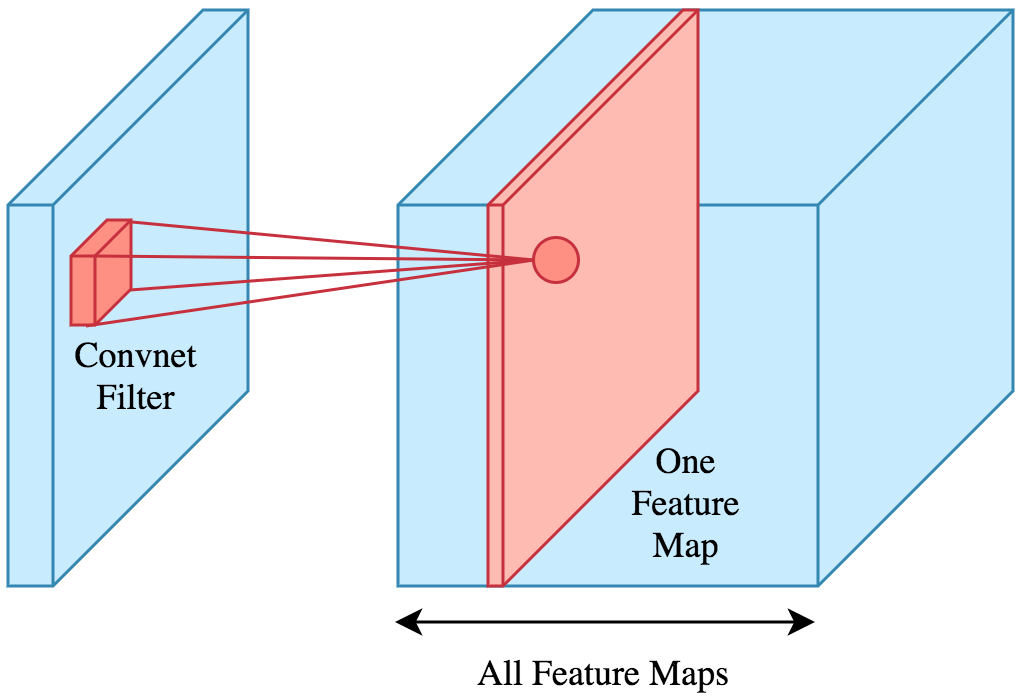
\includegraphics[width=0.5\textwidth]{chapters/chapter3/images/cnn.png}
	\caption{Single convolutional layer using filters
		\label{fig:single-cnn-layer}
	}
\end{figure}

In addition, CNNs can exploit the spatial structure of the data by using different building blocks in order to construct the network. Some of the layers help to avoid problems such as overfitting which is a key problem when training these networks. Others such as ReLU layers help reduce the training time since it simplifies the activation functions with having too much impact on the overall network accuracy. Below is a list of a the most common layers used in CNNs with a short explanation the role of each.

\begin{itemize}
	\item Convolution. Layer with filters that have learnable weights. Computing output is dot product of each filter with the input.
	\item Pooling. Layer that acts as non-linear downsampling of the input. Helps control overfitting by reducing size of network and number of learnable parameters.
	\item ReLU. Layer which applies an activation function to the input of the layer that removes negative values from the input by setting to those values to zero. \cite{Romanuke2017} Improves speed of training the network.
	\item Fully-connected. At the end of the network, a fully-connnected layer can be added in order to perform high-level decisions such as predicting MNIST digits. This is usually an MLP (described in Section \ref{dsgn:sec:dl:mlp}).
\end{itemize}

By carefully combining these different layers, we form a convolutional neural network. The main applications are in image recognition and visual processing such as images and video; in this project we a CNN is used to process frames from Atari. As previously touched upon in Section \ref{bg:sec:cnn-vis}, we can view what information the network has chosen to learnt by looking at the activation in each layer, and each filter. It can provide insight into how well the network is learning and if it requires fine-tuning.

Figure \ref{fig:mnist-arch} provides an example network that is used to predict the value of a hardwritten digit from the MNIST\footnote{\href{http://yann.lecun.com/exdb/mnist/}{MNIST}. Large database of 60,000 training image of 28x28 images showing hardwritten digits from 0-9} dataset. It uses a series of convolution (CONV) and pooling (POOL) layers before connnecting to a fully-connected network (with 10 outputs) which is used to perform the final prediction of the number.

\begin{figure}[htbp]
	\centering
	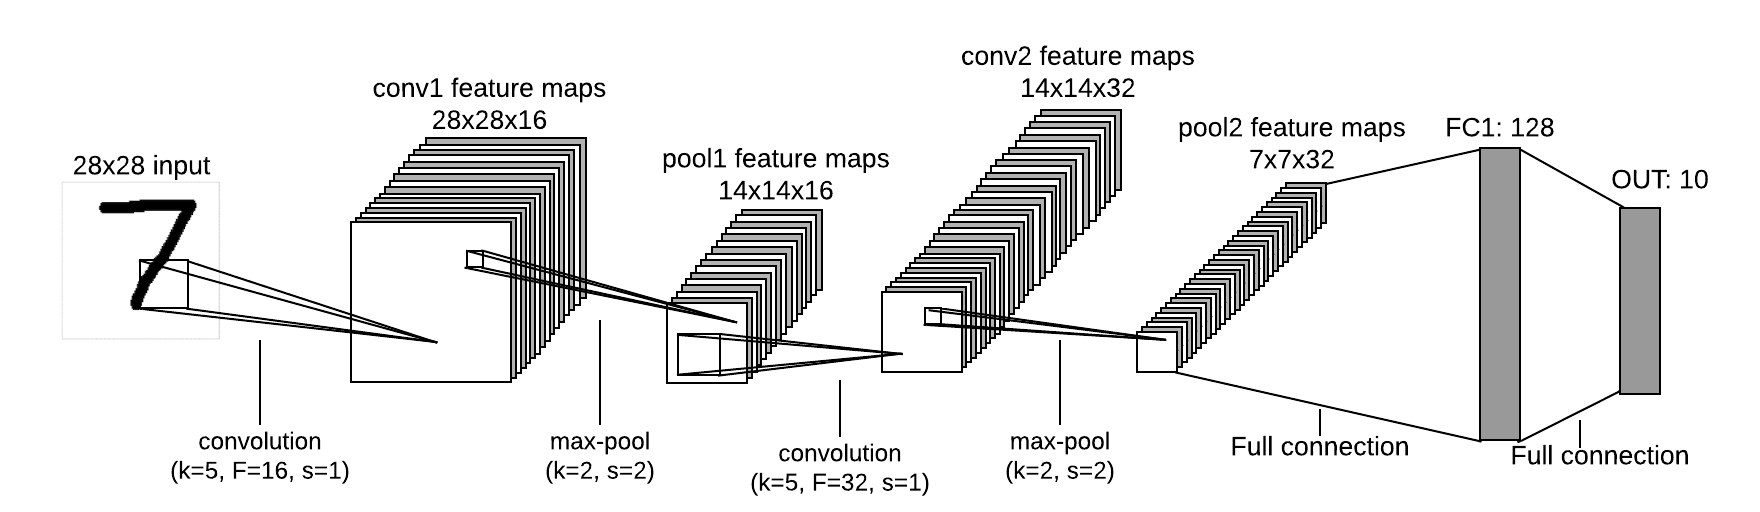
\includegraphics[width=0.75\textwidth]{chapters/chapter3/images/mnist.png}
	\caption{Architecture of a network to predict MNIST digits
		\label{fig:mnist-arch}
	}
\end{figure}

\section{Deep Q-Learning}
\label{dsgn:sec:dql}
The following sections will outline how the previous sections have laid the foundation for introducing Deep Q-Learning. It is the method by which the computer can learn to play the Atari games to human-level. It will use the information from the previous sections and also introduce some new concepts such as Experience replay which is key to the learning process.

In this project we use neural networks as the function aprroximator for $Q(s, a)$, we represent this by using $\theta$ to represent the parameterisation of the Q-function, $Q(s, a; \theta)$. Referring back to Section \ref{dsgn:sec:mdp}, the aim of Q-learning is to find a function $Q(s, a; \theta)$ that closely approximated the optimal action-value function $Q_*(s, a)$.
The \textit{value iteration} algorithm will converge to the optimal action-value function, $Q_i \rightarrow Q_*$ as $i \rightarrow \infty$ \cite{richardsutton2018}. In practise however, we need to use a function approximator as it can generalise the solution, given by $Q(s, a; \theta) \approx Q_*(s, a)$.

In order to train the network, we need to define the `loss' function for the Q-function. This will allow us to update the weights of the network in the direction of the gradient, bringing the Q-function closer to $Q_*(s, a)$ with every timestep.

\begin{defn}
	The loss function of the Q-network is defined by
	\[
		L_i(\theta_i) = \mathbb{E}\left[(y_i - Q(s, a; \theta_i))^2\right]
	\]
\end{defn}
where $y_i = \mathbb{E}\left[r + \gamma \max_{a'}Q(s', a'; \theta_{i - 1})\vert s, a\right]$ is the target value for iteration $i$ and the function $L_i(\theta_i)$ is updated at every timestep. It is also important to note that we hold the parameters of the network fixed from the previous iteration $\theta_{i - 1}$ in order to stabilize learning.

By differentiating the loss function defined above, with respect to the weights of the network ($\theta$), we get the following gradient.

\begin{defn}
	\[
		\nabla_{\theta_i} L_i(\theta_i) = \mathbb{E} \left[ \left( r + \gamma \max_{a'} Q(s', a'; \theta_{i - 1}) - Q(s, a; \theta_i)\right) \nabla_{\theta_i} Q(s, a; \theta_i) \right]
	\]
\end{defn}

In practise, when implementing the Q-learning algorithm, it is more computationally efficient to not compute the ful expectation of the graident, rather we optimise the loss using stoachastic graident descent. This leads us onto the Deep Q-Learning algorithm which is presented below.

\begin{algorithm}[H]
	\SetAlgoNoLine
	\DontPrintSemicolon
	Initialize replay memory $\mathcal{D}$ with maximum capacity $N$\;
	Initialize action-value function $Q$ with random weights $\theta$\;
	Initialize \textbf{target} action-value function $\hat{Q}$ with weights $\theta_{}^{-} = \theta$\;
	\For{timestep = 1, T}{
		Initialise S\;
		\While{S is not done state}{
			With probability $\varepsilon$ choose random action $a_t$\;
			otherwise, pick $a_t = \max_{a}Q(s_t, a;~\theta)$\;
			Take action $a_t$ and observse reward $r_t$ and state $s_{t + 1}$\;
			Pre-process the state $s_{t + 1}$ as $\phi_{t + 1} = \phi(s_{t + 1})$\;
			Store tuple $(\phi_{t}, a_t, r_t, \phi_{t + 1})$ in $\mathcal{D}$\;
			Randomly sample a minibatch of tuples $(s_i, a_i, r_i, s_{i + 1})$ from $\mathcal{D}$\;
			Set $y_i = \begin{cases}
					r_i,                                                            & \text{if episode done at}~i + 1, \\
					r_i + \gamma \max_{a'}\hat{Q}(\phi_{i + 1},~a';~\theta_{}^{-}), & \text{otherwise}.
				\end{cases}$\;
			Perform gradient descent on $\left( y_i - Q(\phi_i,~a_i;~\theta)\right)^2$ wrt. $\theta$\;
			Every $C$ steps copy weights $\theta_{}^{-} = \theta$
		}
	}
	\caption{Deep Q-Learning with Experience replay}
	\label{algo:dqn}
\end{algorithm}

\subsection{Experience Replay}
\label{dsgn:subsec:exp-replay}

One of the problems with the Q-learning algorithm is that if we try and learn from consecutative frames, the algorithm will take a long time to converge. This is due to the large correlation between consecutative frame of the Atari games. By splitting up the training samples it breaks this correlation and reduces the variance of the gradient updates.

This approach is known as ``\textit{experience replay}'' \cite{Lin1992ReinforcementLF}. Every timestep, we store the tuple $e_t = (s_t, a_t, r_t, s_{t+1})$ of experience in the replay memory which is denoted by $D$ in Algorithm \ref{algo:dqn}. Therefore, over time we accumulate a collection of experiences such that $D = e_1, e_2, \hdots, e_N$.

In practise, we keep a rolling collection of experiences for a memory with capacity N; in this project the experience is stored in a Double-Ended Queue\footnote{Double-ended queue is an abstract data type that can generalise a queue. It typically provides operations to add/remove elements from the head and tail.}. It means that at timestep $N+1$, we remove the tuple $e_1$ and replace it with tuple $e_{N+1}$.

During the Q-learning updates, we take a mini-batch of samples, $e \sim D$, randomly from the replay memory in order to perform the stoachastic gradient descent. This method comes with several benefits that are outlined below.

\begin{itemize}
	\item We randomly sample the replay memory at each step, we can reuse experience samples multiple times, providing much greater data efficiency.
	\item As mentioned previously, there is a strong correlation between consecutative frames, experience replay provides a method to remove this correlation.
\end{itemize}

Despite the benefits that experience replay brings, this approach has limitations. The main being that each experience sample is treated with the same importance i.e. each tuple has an equal probability of being chosen in a sample $e$. Therefore, in 2015 Schaul et al. \cite{per} introduced a new method called ``Prioritized Experience Replay'' which aimed to ensure that more important experiences are replayed with a greater frequency.

\section{Q-Learning improvements}
\label{dsgn:sec:qlearning:qextra}
As discussed in Section \ref{dsgn:sec:dql}, due to how Q-learning works, it can lead to an overestimation of the quality of some actions. Therefore, this section describes two different approaches in order to improve upon the algorithm and reduce the maximisation bias and thereby improving the stability of learning.

\subsection{Double Q-Learning}
\label{dsgn:sec:qlearning:doubledqn}
In the original Q-learning algorithm, experiemental results have shown that under certain conditions the algorithm tends to overestimate the quality of some actions. Therefore, in order to reduce the bias, H. V. Hasselt introduced the double Q estimator function in his 2010 paper \cite{double-ql}. It presents an off-policy reinfrocement learning algorithm where we use two Q-functions, one for the value evaluation and the other for selecting the next action.

\begin{defn}
	Double Q-Learning update equation where
	\[
		Q_{t+1}^A (s_t, a_t) = Q_t^A (s_t, a_t) + \alpha_t \left( R_t + \gamma~Q_t^B \left( s_{t + 1}, \argmax_a Q_t^A (s_{t + 1}, a) \right) - Q_t^A (s_t, a_t) \right) ,
	\]

	and
	\[
		Q_{t+1}^B (s_t, a_t) = Q_t^B (s_t, a_t) + \alpha_t \left( R_t + \gamma~Q_t^A \left( s_{t + 1}, \argmax_a Q_t^B (s_{t + 1}, a) \right) - Q_t^B (s_t, a_t) \right) .
	\]
\end{defn}

This definition means that the estimated value of future rewards is calculated using a different policy, solving the original overestimation issue with Q-learning. An additional note is that although this prevents the overestimation, it can lead to underestimation of the Q-values in some situations.

For this project, we use double Q-learning in combination with deep learning. As proposed by H. V. Hasselt et al. (2015) \cite{deep-double-qlearning}, the original Double Q-Learning algorithm can be simpilifed to only need minor changes to the DQN algorithm in order to achieve a similar effect in reducing the overestimation.

This means that rather than maintaining two different networks, use the target Q-network and fixed network in order to determine the best action to take given a state.
TODO

\subsection{Duelling Q-Learning}
\label{dsgn:sec:qlearning:dueldqn}

This section will describe another improvement to the original Q-learning algorithm that makes changes to the underlying network architecture in order to improve approximation of $q_*(s, a)$. The architecture was first proposed by Z. Wang et al, 2015 \cite{wang2015dueling}.

By using Definition \ref{action-value-func} and Definition \ref{state-value-func} we can define a quantity called the Advantage, denoted by $A_\pi(\cdot, \cdot)$.

\begin{defn}
	\label{advantage-func}
	The \textit{advantage function} relates the Q and value functions.

	\[
		A_\pi(s,~a) = Q_\pi(s,~a) - V_\pi(s)
	\]
\end{defn}

In order to know what quantity the advantage funnction produces, recall that the Q-function describes the quality of taking an action $a$ in state $s$, and that the value function describes how good it is to be in a state $s$. Therefore, since the advantage function subtracts the value of a function from the Q-function, it obtains a relative measure of the importance of each action $a$ in state $s$.

\begin{figure}[htbp]
	\centering
	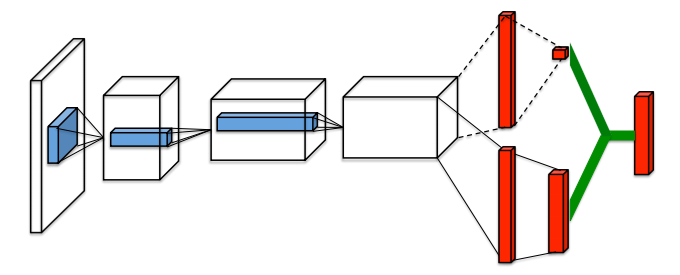
\includegraphics[width=0.75\textwidth]{chapters/chapter3/images/duelling.png}
	\caption{Duelling Q-Network architecture
		\label{fig:duelling-arch}
	}
\end{figure}

As shown above, rather than having a single fully-connnetced layer than predicts a Q-value for each output (like in Section \ref{dsgn:sec:dql}), the Duelling Q-Network maintains two discrete paths. One path attempts to predict the function $V_\pi(s)$, the other predicts $A_\pi(s, a)$. Finally, these two paths are combined together to calculate $Q_\pi(s, a)$. It is important to note, this is not an extra step in the training process, rather, it is built directly into the network and calculated during a forward pass. This is represented by the green lines combining the two paths to the output layer in Figure \ref{fig:duelling-arch}.

\begin{defn}
	Q-function combining advantage and value functions

	\[
		Q(s, a; \theta, \alpha, \beta) = V(s, a; \theta, \beta) + \left( A(s, a; \theta, \alpha) - \frac{1}{A} \sum_{a'\in A} A(s, a; \theta, \alpha) \right)
	\]
\end{defn}

As the above defintion shows we calculate estimates of the Q-values for each action, and choosing the best action requires finding $a_* = \argmax_{a' \in A} Q(s, a; \theta)$. $\alpha$ and $\beta$ are the parameters for the value and advantage functions respectively.

In order to calculate the Q-function, it would be intuitive to perform the arithmatic sum of the value and advantage function based on Definition \ref{advantage-func}, however, using that method leads to two problems \cite{wang2015dueling}.

\begin{itemize}
	\item It can be problimatic to assume the functions give good estimates of the true values, especially using parameterised versions of the functions
	\item Naive sum of two values is `unidentifiable'. Given a Q-value, we cannot recover $V_\pi(\cdot)$ and $A_\pi(\cdot, \cdot)$ uniquely
\end{itemize}

This architecture has shown to achieve best in-class performance over the different methods that are described in the sections above. In addition, these methods don't have to be used in isolation, some of the methods can be combined to further improve the performance of the Deep Q-Networks. For example, this project uses a Duelling Double Q-network architecture which outperforms the basic DQN since it is much more stable and prevents the overestimation problem.


% this causes the references to be listed
\bibliography{refs}

% this determines the style in which the references are printed,
% other possible values are plain and abbrv
\bibliographystyle{abbrv}

%% Appendices start here
\appendix
%\chapter{Example of operation}

An appendix is just like any other chapter, except that it comes after
the appendix command in the master file.

One use of an appendix is to include an example of input to the system
and the corresponding output.

One way to do this is to include, unformatted, an existing input file. 
You can do this using \verb=\verbatiminput=. In this appendix we
include a copy of the C file \textsf{hello.c} and its output file
\textsf{hello.out}. If you use this facility you should make sure that
the file which you input does not contain \texttt{TAB} characters,
since \LaTeX\ treats each \texttt{TAB} as a single space; you can use
the Unix command \texttt{expand} (see manual page) to expand tabs into
the appropriate number of spaces. 

\section{Example input and output}
\label{sec:inp-eg}
\subsection{Input}
\label{sec:input}
(Actually, this isn't input, it's the source code, but it will do as
an example)

\verbatiminput{hello.c}

\subsection{Output}
\label{sec:output}

\verbatiminput{hello.out}
\subsection{Another way to include code}
You can also use the capabilities of the \texttt{listings} package to
include sections of code, it does some keyword highlighting.

%\lstinputlisting[language=C]{hello.c}

% Local Variables: 
% mode: latex
% TeX-master: "report"
% End: 


\end{document}
